\renewcommand\thetable{\arabic{chapter}-\arabic{table}}
%\renewcommand\thefigure{\arabic{chapter}-\arabic{figure}} 
\chapter{結論與未來展望}
\label{cha:conclusions}

\section{結論}

教育部所主持的「加速高中職及國中小老舊校舍及相關設備補強整建計畫」以及其相關的後續計畫,在執行上和一般的計畫一樣會受到預算的限制,但是此一計畫的預算限制直接的影響到能夠改善多少校舍的耐震能力,因此如何有效的估計校舍詳細評估、補強的預算需求,並正確的挑選出應該優先處理的校舍對於學生的生命安全關係重大,然而實際上校舍補強的正確經費是在計畫非常後期才會得到,因此在每個年度的一開始,計畫的執行人員都要透過經驗公式來推估待評估的校舍需要多少經費來評估和補強,雖然此一經驗公式也有一定程度的可靠度,但是其尚缺乏理論支持。

需要補強的校舍在得知實際的補強經費之前,會先經過初步評估、詳細評估和補強設計幾個階段的作業,然後才是實際的補強施工,本研究目前的成果也是分佈在此一程序上的不同位置,包括了初步評估的~$Is$~值關係模型、詳細評估的~$CDR$~值關係模型、詳細評估的破壞構件關係模型、以及最後的校舍補強經費關係模型,其關係如圖~\ref{fig:FLOW-con}~所示。
其中,校舍群集模型被用作其它資料探勘的資料前處理的其中一項,因此較難直接瞭解其模型品質,然而使用此一群集模型後分別建立不同得關係模型所得到的結果確實較好;而使用此一群集模型所得到的初步評估~$Is$~值與校舍基本設計參數間的關係模型,其~$R^2$~達到了~0.76~;更進一步的詳細評估的~$CDR$~值與校舍基本設計參數間的關係模型,使用~WGP~方法建立出來,其~RMSE~為~0.039,也達到了國震中心專家所建議的~0.04~以下的目標;而詳細評估後的構件破壞情形的模型,也有很不錯的表現,五種構件均有~75\%~以上的正確率,其中~RC~牆、磚牆和柱的關係模型更是有~80\%~以上;流程最後的校舍補強經費與校舍基本設計參數間的關係模型,表現較為一般,其~$R^2$~為~0.69~,然而如果考量到此模型在實務上應用之方式,則可使用平均誤差判斷模型品質,而此模型的平均誤差表現非常好,235~棟校舍之誤差僅有~11066~元,而一棟校舍平均的補強經費則高達~400~多萬,誤差約為~0.26\%~。

\begin{figure}[hbtp]
  \begin{center}
    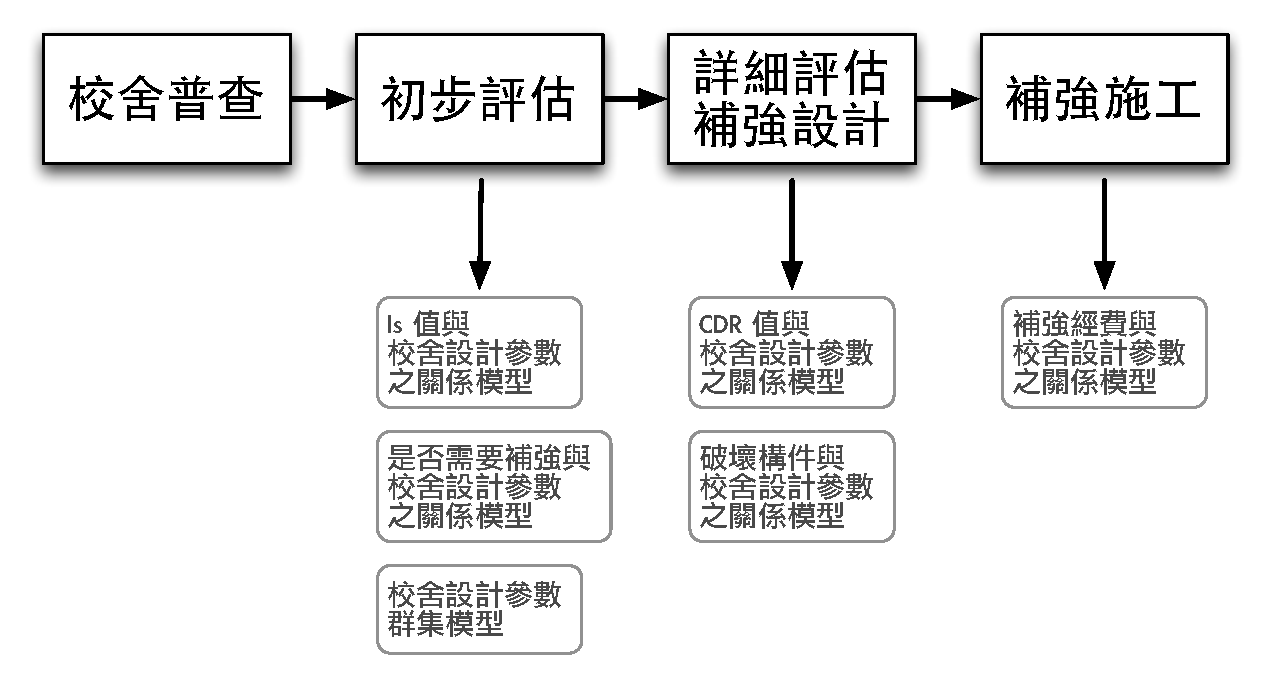
\includegraphics[width=1.0\textwidth]{figures/survey-flow-con.pdf}
    \caption{評估流程與資料探勘模型} 
    \label{fig:FLOW-con}
  \end{center}
\end{figure}

本研究所提出數個基於校舍耐震資料庫與資料探勘方法所得到的關係模型,均有不錯的表現,而這些關係模型的目標屬性均是校舍耐震能力補強計畫的工作流程中,不同階段的產出,透過這些關係模型,可以快速的得到本來是非線性關係,不容易取得的關鍵屬性,並且保有一定程度的可靠性,這些模型雖然無法直接的取代現有的評估流程,但是其知識之內容相信可以輔助整個校舍耐震能力補強計畫的工作,例如:藉由~$Is$~值的關係模型來判斷一群校舍整體的耐震能力表現、甚至是可以直接使用補強經費得關係模型來輔助決策者,判斷要編列多少預算,並且可以同時瞭解到這些預算可以完成多少校舍的補強、這些校舍佔所有耐震能力有疑慮的校舍中的比例,甚至是反過來,根據決策者決定要補強多少棟或是多少比例的校舍,再透過關係模型計算這些校舍的總補強經費為多少,提供給決策者做參考。這些應用都可以有效的提升校舍耐震能力補強作業的效能,讓主事者更快的瞭解校舍的狀況,並且更有效的分配預算。

\section{未來展望} 

本論文目前之主要之成果為耐震能力與補強預算相關之知識,然而本研究初期時即依照資料探勘的四種知識類型:迴歸、分類、分群、關聯分別分析設計了數個不同面像的探勘目標如圖~\ref{fig:bigpicture}~,分別詳述如下:

\begin{description}
  \item[迴歸]
  主要的知識為重要屬性的關係模型,且要為數值類型的屬性,例如校舍的最小破壞地表加速度、耐震能力、補強經費等。
  \item[分類]
  分類探勘類型的知識和迴歸類之知識相似,主要也是用在建立重要屬性的關係模型,其主要差異在於迴歸分析僅能對數值類型之屬性建立模型,而分類分析則僅能對資料數值為集合類之屬性建立模型,目前所設計之分析為校舍是否安全、是否需要補強的分類分析。
  \item[分群]
  分群類型之知識主要在於校舍結構之不同群集,其知識之形式與分類分析有些相似,最大之不同點在於此類模型在訓練建立時,並沒有輸出參數,而是只靠輸入參數間來判斷資料間的相似度,例如相似結構形式的校舍群集,組成校舍的結構元件的探勘等。
  \item[關聯]
  此類型之知識形式為屬性間的特殊關係,例如特定年代的校舍在設計上會有不同於其他年代的的形式,而這些特色如果可以在典型校舍的設計參數上表現出來,應當可以用此種資料探勘尋找出來,而預期的目標包括了不同年代校舍之設計特色、校舍結構之設計模式等。
\end{description}

\begin{figure}[hbtp]
  \begin{center}
    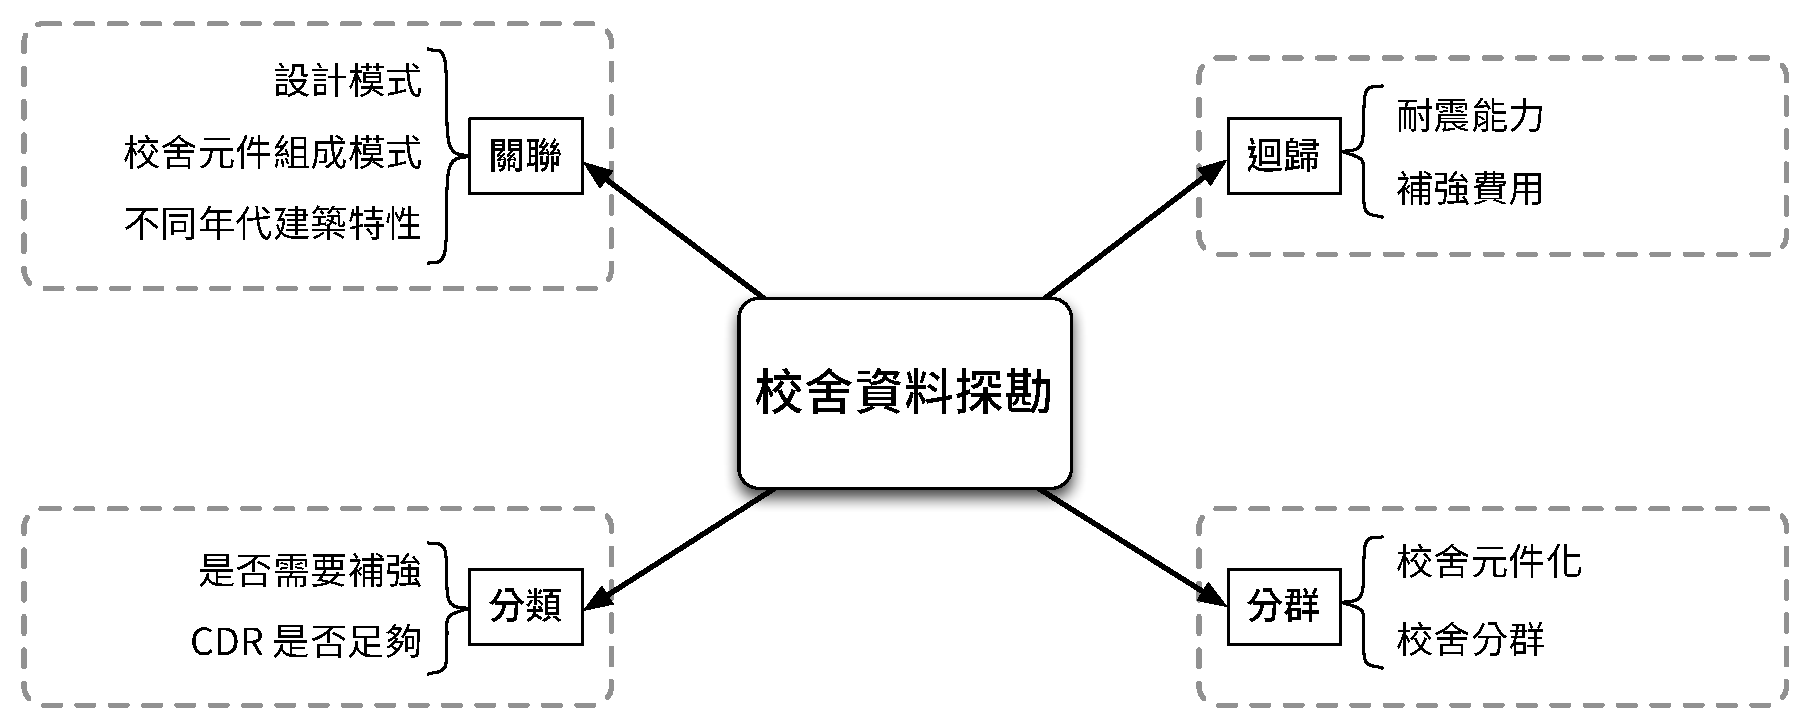
\includegraphics[width=1.0\textwidth]{figures/big-picture.pdf}
    \caption{知識挖掘規劃} 
    \label{fig:bigpicture}
  \end{center}
\end{figure}

本研究目前透過資料探勘所得到之知識,均分佈在教育部的校舍耐震能力補強的流程之上,包括了分類形式的校舍是否需要補強與其設計參數之關係模型、迴歸形式的校舍耐震能力與其設計參數之關係模型以及校舍補強經費與其設計參數之關係模型、還有分群形式的校舍群集模型,其在建立耐震能力關係模型時,作為資料前處理輔助用。而第一個發展方向,就是更進一步往不同的方向進行資料探勘,例如初期規劃所設計的探勘目標,在關聯形式的知識尚沒有任何可用的成果,但是研究初期規劃的那些知識隱含於耐震資料庫中的可能性極高,而且這類知識的發掘雖然無法直接回饋到校舍耐震補強計畫之上,但是卻可能在其它的校舍相關議題上發揮其功用。

% 主要都是以輔助目前的校舍耐震能力補強計畫流程作為出發點

% 在本研究中,建立校舍設計參數與其~$Is$~值之關係模型時,便有使用到此一知識來增進關係模型的品質,後續研究還可以針對這些校舍群集,進一步分析其不同群集之特性,至於關聯形式的知識,本研究目前尚未有可用的知識產出,因此後續的研究方向也包含此一類型知識的探勘與挖掘。

第二個發展方向,則是可以嘗試將目前獨立分佈在耐震能力補強流程上的數個資料探勘也串接起來,由於目前資料的複雜度的關係問題,不同的資料探勘分析都是獨立進行分析,包括資料前處理的資料篩選也是根據問題的特性來調整,因此不同的模型所需要的輸入資料的屬性,雖然有很大程度是相關的屬性,但是仍有差異,也造成判斷校舍是否需要補強的的輸入資料集無法用讓~$CDR$~值關係模型的來使用,$CDR$~值關係模型的輸入資料集也無法用作補強經費關係模型的輸入之用。但是也因為不同模型的輸入資料屬性有很大的相關度,那也表示應該可以探討出一組資料屬性集,同時可以找出和初步評估的~$Is$~值、詳細評估的~$CDR$~值以及補強校舍的補強經費都能夠找出其關係模型,那麼應該可以用這組模型,在校舍建築物調查非常初始的階段,就能夠推估它的耐震能力表現如何、是否足夠,進一步到是否需要補強、補強經費多少。

最後一個發展方向,則是在~CRISP-DM~流程當中的最後一個步驟,將探勘得到的知識實際回饋到學校校舍及相關設備的補強整建計畫上,由於目前探勘得到的知識都還是以數學模型的形式存在,非專業人士難以應用,因此如果可以將這些數學模型轉化成決策支援系統,則可以讓主管機關能夠簡單的得到這些模型的輔助,在校舍長期持續的耐震能力監控上,能夠發揮探勘所得知識的效力。





